% BEGIN LICENSE BLOCK
% Version: CMPL 1.1
%
% The contents of this file are subject to the Cisco-style Mozilla Public
% License Version 1.1 (the "License"); you may not use this file except
% in compliance with the License.  You may obtain a copy of the License
% at www.eclipse-clp.org/license.
%
% Software distributed under the License is distributed on an "AS IS"
% basis, WITHOUT WARRANTY OF ANY KIND, either express or implied.  See
% the License for the specific language governing rights and limitations
% under the License.
%
% The Original Code is  The ECLiPSe Constraint Logic Programming System.
% The Initial Developer of the Original Code is  Cisco Systems, Inc.
% Portions created by the Initial Developer are
% Copyright (C) 1994 - 2006 Cisco Systems, Inc.  All Rights Reserved.
%
% Contributor(s):
%
% END LICENSE BLOCK
%
% @(#)umsusing.tex	1.10 94/12/06
%
% \comment{@(\#)text1.mss	20.4 9/19/88}
%
% REL	DATE	BY		DESCRIPTION
% 2.10	260489	David Miller	Convert to LaTeX and update
%

\newcommand{\guitext}[1]{\mbox{\texttt{#1}}}
\newcommand{\keyboard}[1]{{\texttt{#1}}}
%\newcommand{\menu}[1]{{\texttt{#1}}}
%\newcommand{\menuopt}[1]{{\texttt{#1}}}
%\newcommand{\button}[1]{{\texttt{#1}}}
\newcommand{\menu}[1]{\guitext{#1}}
\newcommand{\menuopt}[1]{\guitext{#1}}
\newcommand{\button}[1]{\guitext{#1}}

\newcommand{\ignore}[1]{}

%------------------------------------------------------------------------
\chapter{Getting started with {\eclipse}}
%HEVEA\cutdef[1]{section}
%------------------------------------------------------------------------
\label{chapusing}

%------------------------------------------------------------------------
\section{How do I install the {\eclipse} system?}
%------------------------------------------------------------------------
Please see the installation notes that came with {\eclipse}.
For Unix/Linux systems, these are in the file \notation{README_UNIX}.
For Windows, they are in the file \notation{README_WIN.TXT}.

Please note that choices made at installation time can affect which options
are available in the installed system.

%------------------------------------------------------------------------
\section{How do I run my {\eclipse} programs?}
%------------------------------------------------------------------------
There are two ways of running {\eclipse} programs.
The first is using \notation{tkeclipse}, which provides an interactive graphical
user interface to the {\eclipse} compiler and system.
The second is using \notation{eclipse}, which provides a more traditional
command-line interface.
We recommend you use {\tkeclipse} unless you have some reason to prefer a
command-line interface.

%------------------------------------------------------------------------
\section{How do I use \notation{\tkeclipse}?}
%------------------------------------------------------------------------

\subsection{Getting started}

To start {\tkeclipse}, either type the command \notation{tkeclipse} at an
operating system command-line prompt, or select {\tkeclipse} from the
program menu on Windows.
This will bring up the {\tkeclipse} top-level, which is shown in
Figure~\ref{tktop}.

\begin{figure}[bt]
\begin{center}
% funny pathname because this chapter gets included from tutorial as well
\resizebox{0.8\textwidth}{!}{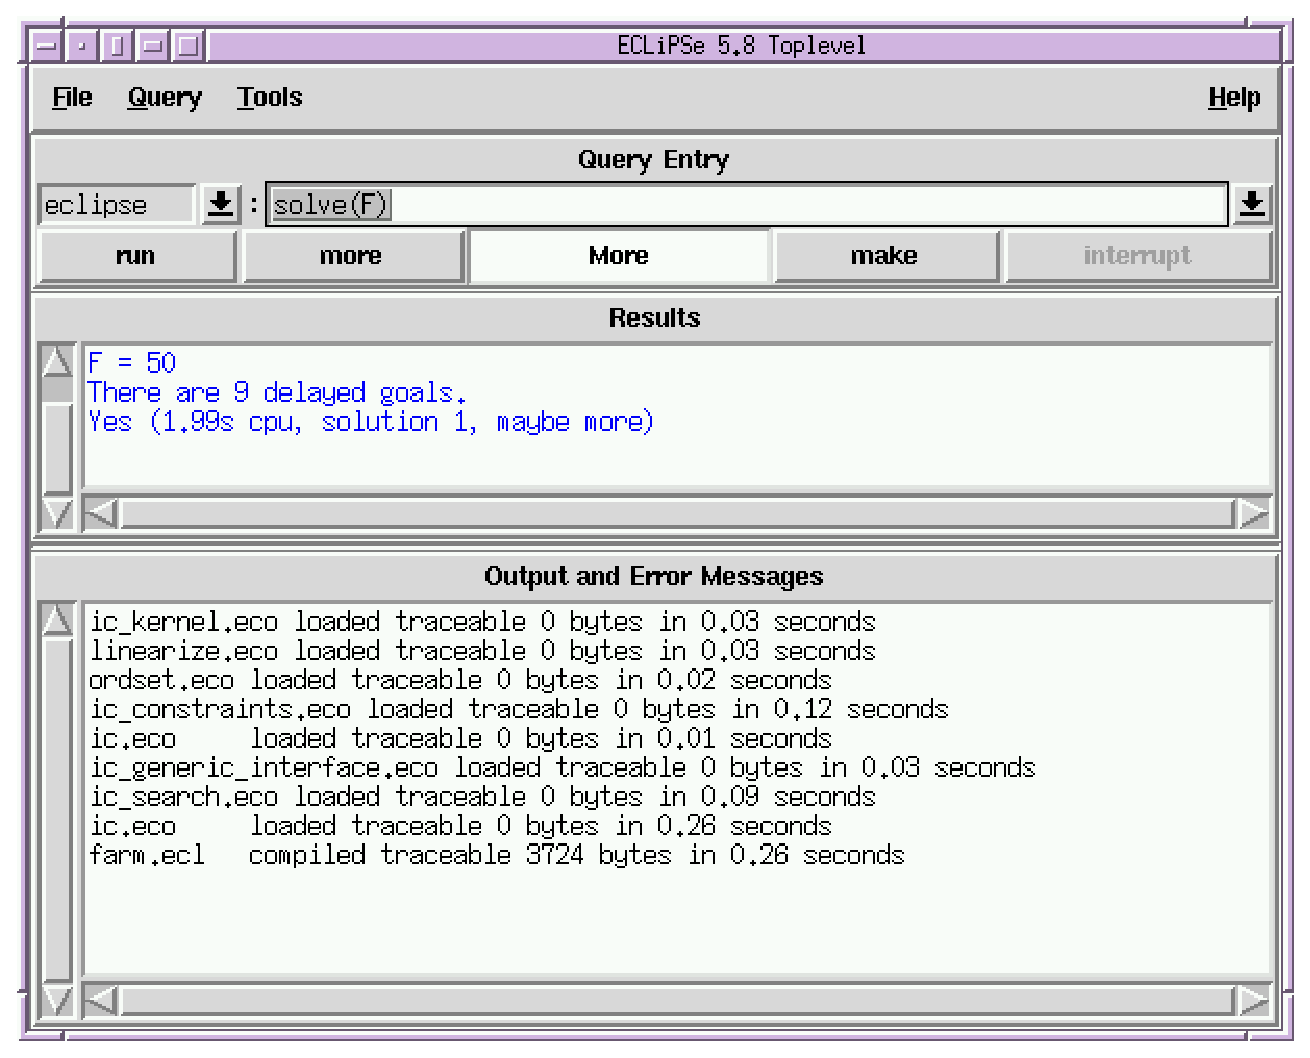
\includegraphics{tktop.eps}}
\end{center}
\caption{{\tkeclipse} top-level}
\label{tktop}
\end{figure}

Note that help on {\tkeclipse} and its component tools is available from the
\menu{Help} menu in the top-level window.
If you need more information than can be found in this manual, try looking
in the \menu{Help} menu.

%------------------------------------------------------------------------
\section{How do I write an {\eclipse} program?}
%------------------------------------------------------------------------
You must use an editor to write your programs. {\eclipse} does not come
with an editor, but any editor that can save plain text files can be used.
Save your program as a plain text file, and you can then compile the
program into {\eclipse} and run it.

With {\tkeclipse}, you can specify the editor you want to use, and this
editor will be started by {\tkeclipse}, e.g., when you select a file in
the `Edit' option under the File menu. The default values are the value of
the VISUAL environment variable  under Unix, or Wordpad under Windows.
This can be changed with the Preference Editor under the Tools menu.

%------------------------------------------------------------------------
\subsection{Compiling a program}

From the \menu{File} menu, select the \menuopt{Compile ...} option.
This will bring up a file selection dialog.
Select the file you wish to compile, and click on the \button{Open} button.
This will compile the file and any others it depends on.
Messages indicating which files have been compiled and describing any errors
encountered will be displayed in the bottom portion of the {\tkeclipse}
window (\guitext{Output and Error Messages}).

If a file has been modified since it was compiled,
it may be recompiled by clicking on the \guitext{make} button.
This recompiles any files which have become out-of-date.

For more information on program compilation and the compiler, please see
chapter \ref{chapcompiler}.

%------------------------------------------------------------------------
\subsection{Executing a query}

To execute a query, first enter it into the \guitext{Query Entry}
text field.
You will also have to specify which module the query should be run from, by
selecting the appropriate entry from the drop-down list to the left of the
\guitext{Query Entry} field.
Normally, the default selection of \guitext{eclipse} will be fine; this will
allow access to all {\eclipse} built-ins and all predicates that have not
explicitly been compiled into a different module.
Selecting another module for the query is only needed if you wish to call a
predicate which is not visible from the \notation{eclipse} module, in which
case you must select that module.
(For more information about the module system, please see chapter
\ref{chapmodules}.)

To actually execute the query, either hit the \keyboard{Enter} key while
editing the query, or click on the \guitext{run} button.
{\tkeclipse} maintains a history of commands entered during the session, and
these may be recalled either by using the drop-down list to the right of the
\guitext{Query Entry} field, or by using the up and down arrow keys while
editing the \guitext{Query Entry} field.

If {\eclipse} cannot find a solution to the query, it will print \notation{No}
in the \guitext{Results} section of the {\tkeclipse} window.
If it finds a solution and knows there are no more, it will print it in the
\guitext{Results} section, and then print \notation{Yes}.
If it finds a solution and there may be more, it will print the solution
found as before, print \notation{More}, and enable the \guitext{more} button.
Clicking on the \guitext{more} button tells {\eclipse} to try to find
another solution.
In all cases it also prints the total time taken to execute the query.

Note that a query can be interrupted during execution by clicking on the
\guitext{interrupt} button.

%------------------------------------------------------------------------
\subsection{Editing a file}
\label{secedit}

If you wish to edit a file (e.g., a program source file), then you may do so
by selecting the \guitext{Edit ...} option from the \guitext{File} menu.
This will bring up a file selection dialog.
Select the file you wish to edit, and click on the \guitext{Open} button.

When you have finished editing the file, save it.
After you've saved it, if you wish to update the version compiled into
{\eclipse} (assuming it had been compiled previously), simply click on the
\guitext{make} button.

You can change which program is used to edit your file by using the
{\tkeclipse} Preference Editor, available from the \guitext{Tools} menu.

%------------------------------------------------------------------------
\subsection{Debugging a program}
\label{secdebug}

To help diagnose problems in {\eclipse} programs, {\tkeclipse} provides the
tracer.
This can be invoked by selecting the \guitext{Tracer} option from the
\guitext{Tools} menu.
The next time a goal is executed, the tracer window will become active,
allowing you to step through the program's execution and examine the
program's state as it executes.

The tracer displays the current call stack, the program source, and a trace log.
By using the left mouse button in the \guitext{Call Stack} region of the
tracer window, you can bring up a menu of additional operations you can
perform on that goal, such as inspecting it, or setting a spy point on the
predicate in question.  Source breakpoints can be set by marking the
corresponding line in the tracer's source display.
Selecting \guitext{Configure filter ...} from the \guitext{Options} menu
of the tracer will launch the conditional filter.
This filter allows you to
specify conditions on which the tracer should stop at a debug port. This
can be very useful for skipping over unwanted debug ports.

For more information on using the tracer, please see the online help,
available by selecting \guitext{Tracer Help} from the \guitext{Help} menu.

Other {\tkeclipse} tools which are useful while using the tracer are:

\begin{itemize}

\item the predicate browser (available by selecting the \guitext{Predicate
Browser} option from the \guitext{Tools} menu), which is useful for setting
or removing spy points on predicates, or for setting the
\notation{start_tracing}
flag which activates the tracer when a particular predicate is called for
the first time; and

\item the term inspector (available by double left clicking on a term from
the stack window, or by selecting the \guitext{Inspector}
option from the \guitext{Tools} menu), which is useful for examining and
browse the arguments of a term in detail.

\item the delayed goals browser (available by selecting the \guitext{Delayed
Goals} option from the \guitext{Tools} menu), which allows you to inspect
the current list of delayed goals.

\item the display matrix (available either from calls in user's code, or by
interactively selecting terms to be observed from the inspector, tracer or
delay goals tools), which allows you to monitor any changes to a term and
its arguments.

\end{itemize}

More information about debugging in {\eclipse} may be found in chapter
\ref{chapdebug}.

%------------------------------------------------------------------------
\subsection{Getting help}

More detailed help than is provided here can be obtained online.
Simply select the entry from the \guitext{Help} menu on {\tkeclipse}'s
top-level window which corresponds to the topic or tool you are interested
in.

%------------------------------------------------------------------------
\subsection{Other tools}

{\tkeclipse} comes with a number of useful tools.
Some have been mentioned above, but here is a more complete list.
Note that we only provide brief descriptions here; for more details, please
see the online help for the tool in question.

\subsubsection{Compile scratch-pad}

This tool allows you to enter small amounts of program code and have it
compiled.
This is useful for quick experimentation, but not for larger examples or
programs you wish to keep, since the source code is lost when the session is
exited.

\subsubsection{Source File Manager}

This tool allows you to keep track of and manage which source files have
been compiled in the current {\eclipse} session.
You can select files to edit them, or compile them individually, as well as
adding new files.

\subsubsection{Predicate Browser}

This tool allows you to browse through the modules and predicates which have
been compiled in the current session.
It also lets you alter some properties of compiled predicates.

\subsubsection{Source Viewer}

This tool attempts to display the source code for predicates selected in
other tools.

\subsubsection{Delayed Goals}

This tool displays the current delayed goals, as well as allowing a spy
point to be placed on the predicate and the source code viewed.

\subsubsection{Tracer}

As discussed in section \ref{secdebug}, the tracer is useful for debugging
programs.
See also chapter \ref{chapdebug}.

\subsubsection{Inspector}

This tool provides a graphical browser for inspecting terms.
Goals and data terms are displayed as a tree structure.
Sub-trees can be collapsed and expanded by double-clicking.
A navigation panel can be launched which provides arrow buttons as an
alternative way to navigate the tree.

Note that while the inspector window is open, interaction with other
{\tkeclipse} windows is disallowed.
This prevents the term from changing while being inspected.
To continue {\tkeclipse}, the inspector window must be closed.

\subsubsection{Global Settings}

This tool allows the setting of some global flags governing the way
{\eclipse} behaves.
See also the documentation for the
\bipref{set_flag/2}{../bips/kernel/env/set_flag-2.html} and
\bipref{get_flag/2}{../bips/kernel/env/get_flag-2.html} predicates.

\subsubsection{Statistics}

This tool displays some statistics about memory and CPU usage of the
{\eclipse} system, updated at regular intervals.
See also the documentation for the
\bipref{statistics/0}{../bips/kernel/env/statistics-0.html} and
\bipref{statistics/2}{../bips/kernel/env/statistics-2.html} predicates.

\subsubsection{Simple Query}

This tool allows the user to send a simple query to {\eclipse} even while
{\eclipse} is running some program and the Toplevel Query Entry window
is unavailable.
Note that the reply is shown in EXDR format (see the {\eclipse} Embedding
and Interfacing Manual).

\subsubsection{Library Help}

This tool allows you to browse the online help for the {\eclipse} libraries.
On the left is a tree display of the libraries available and the predicates
they provide.
\begin{itemize}
\item Double clicking on a node in this tree either expands it or collapses it
again.
\item Clicking on an entry displays help for that entry to the right.
\item Double clicking on a word in the right-hand pane searches for help
entries containing that string.
\end{itemize}
You can also enter a search string or a predicate specification manually
in the text entry box at the top right.
If there is only one match, detailed help for that predicate is displayed.
If there are multiple matches, only very brief help is displayed for each;
to get detailed help, try specifying the module and/or the arity of the
predicate in the text field.

\subsection{Preference Editor}

This tool allows you to edit and set various user preferences. This include
parameters for how {\tkeclipse} will start up, e.g., the amount of memory it
will be able to use, and an initial query to execute; and parameters which
affects the appearance of {\tkeclipse}, such as the fonts {\tkeclipse}
uses.

%------------------------------------------------------------------------
\section{How do I use \notation{eclipse}?}
%------------------------------------------------------------------------

\subsection{Getting started}

To start {\eclipse}, type the command \notation{eclipse} at an
operating system command-line prompt.
This will display something like this:
\begin{quote}
\begin{verbatim}
% eclipse
ECLiPSe Constraint Logic Programming System [kernel]
Kernel and basic libraries copyright Cisco Systems, Inc.
and subject to the Cisco-style Mozilla Public Licence 1.1
(see legal/cmpl.txt or eclipseclp.org/licence)
Source available at www.sourceforge.org/projects/eclipse-clp
GMP library copyright Free Software Foundation, see legal/lgpl.txt
For other libraries see their individual copyright notices
Version X.Y #Z, DAY MONTH DD HH:MM YYYY
[eclipse 1]:
\end{verbatim}
\end{quote}
The list in square brackets on the first line specifies the configuration
of the running system, i.e., the language extensions that are present.
The copyright and version information is followed by the prompt
\notation{[eclipse 1]:}, which tells the user that the top-level loop is waiting
for a user query in the module \notation{eclipse}.
The predicate \predspecidx{help/0} gives
general help and \bipref{help/1}{../bips/kernel/env/help-1.html} gives
help about specific built-in predicates.

%------------------------------------------------------------------------
\subsection{Interacting with the top level loop}

The {\eclipse} prompt \notation{[eclipse 1]:} indicates that {\eclipse}
is at the top level
and the opened module is \notation{eclipse}.
The \aboutidx{top level loop} is a procedure which repetitively
prompts the user for a query, executes it and reports its
result, i.e., either the answer variable bindings or the
failure message.
There is always exactly one module opened in the top level
and its name is printed in the prompt.
From this point it is possible to enter {\eclipse} goals, e.g., to
pose queries, to enter an {\eclipse} program from the keyboard
or to compile a program from a file.
Goals are entered after the prompt and are terminated by fullstop and
newline.

The {\eclipse} system may be exited by typing \notation{CTRL-D} (UNIX) or
\notation{CTRL-Z} + \notation{RETURN} (Windows) at the top level prompt,
\index{Exiting {\eclipse}}
or by calling either the \bipref{halt/0}{../bips/kernel/opsys/halt-0.html}
or the \bipref{exit/1}{../bips/kernel/opsys/exit-1.html} predicates.

%------------------------------------------------------------------------
\subsection{Compiling a program}

The square brackets \notation{[}\pattern{...}\notation{]} or the
\bipref{compile/1}{../bips/kernel/compiler/compile-1.html} predicate are used
to compile {\eclipse} source from a file.
If the goal
\begin{quote}
\begin{verbatim}
compile(myfile).
\end{verbatim}
\end{quote}
or the short-hand notation
\begin{quote}
\begin{verbatim}
[myfile].
\end{verbatim}
\end{quote}
is called, either as a query at the top level or within another goal,
the system looks for the file \notation{myfile} or for a file called
\notation{myfile.pl} or \notation{myfile.ecl} and compiles it.
The short-hand notation may also be used to compile several files in
sequence:
\begin{quote}
\begin{verbatim}
[ file_1, file_2, ..., file_n ]
\end{verbatim}
\end{quote}
The \bipref{compile/2}{../bips/kernel/compiler/compile-2.html} predicate may be
used to compile a file or list of
files into a module specified in the second argument.

If a file has been modified since it was compiled, it may be recompiled by
invoking the \bipref{make/0}{../bips/kernel/env/make-0.html} predicate.
This recompiles any files which have become out-of-date.

For more information on program compilation and the compiler, please see
chapter \ref{chapcompiler}.

%------------------------------------------------------------------------
\subsection{Entering a program from the terminal}

Programs can be entered directly from the terminal, as well as being read
from files.
To do this, simply compile the special file \notation{user}.
That is, \notation{[user].} or \notation{compile(user).} at a top level
prompt.
The system then displays the compiler prompt (which is a blank by default)
and waits for a sequence of clauses.
Each of the clauses is terminated by a fullstop.%
\index{fullstop}\index{clause!termination}
(If the fullstop is omitted the system just sits
waiting, because it supposes the clause is not terminated.
If you omit the fullstop by accident simply type it in on the following line,
and then proceed to type in the program clauses, each followed by a fullstop and
carriage return.)
To return to the top level prompt,
type CTRL-D (UNIX), CTRL-Z + RETURN (Windows) or enter the atom
\notation{end_of_file} followed by fullstop and RETURN.

For example:
\begin{quote}
\begin{verbatim}
[eclipse 1]: [user].
source_processor.eco loaded in 0.01 seconds
...
ecl_compiler.eco loaded in 0.23 seconds
 father(abraham, isaac).
 father(isaac, jacob).
 father(jacob, joseph).
 ancestor(X, Y) :- father(X, Y).
 ancestor(X, Y) :- ancestor(X, Z), ancestor(Z, Y).
 ^D
 tty        compiled 420 bytes in 0.01 seconds

Yes (0.24s cpu)
[eclipse 2]:
\end{verbatim}
\end{quote}
The two predicates \predspec{father/2} and \predspec{ancestor/2} are now
compiled
and can be used.

%------------------------------------------------------------------------
\subsection{Executing a \Index{query}}

Once a set of clauses has been compiled,
it may be queried in the usual Prolog manner.
If there are uninstantiated \Index{variables} in the query,
the system will attempt to find an instantiation of them which will
satisfy the query, and if successful it will
display one such instantiation.
If potentially there is another solution, the top level
will then wait for a further instruction: either a \notation{<CR>}
(``newline'' or ``return'') or a semi-colon (\notation{;}).
A return will end the query successfully.
A semi-colon will initiate \Index{backtracking}
in an attempt to find another solution to the query.
Note that it is not necessary to type a new line after the semicolon
--- one keystroke is enough.
When the top level loop can detect
that there are no further solutions, it does not wait for the semicolon
or newline, but it displays directly the next prompt.
For example in a query on
a family database:
\begin{quote}
\begin{verbatim}
[eclipse 3]: father(X, Y).

X = abraham
Y = isaac
Yes (0.00s cpu, solution 1, maybe more) ? ;            (user types ';')

X = isaac
Y = jacob
Yes (0.00s cpu, solution 2)
[eclipse 4]:
\end{verbatim}
\end{quote}

Queries may be extended over more than one line. When this is done the prompt
changes to a tabulation character, i.e., the input is indented to
indicate that the query is not yet completed.
The fullstop marks the end of the input.

%------------------------------------------------------------------------
\subsection{Interrupting the execution\index{interrupt}}

If a program is executing, it may be interrupted by
typing \notation{CTRL-C} (interrupt in the UNIX environment).
This will invoke the corresponding interrupt handler
(see section \ref{sectinterrupts}).
By default, the system prints a menu offering some alternatives:
\begin{quote}
\begin{verbatim}
^C
interruption: type a, b, c, e, or h for help : ? h       (user types 'h')
help
	a : abort
	b : break level
	c : continue
	e : exit
	h : help


interruption: type a, b, c, e, or h for help : ?
\end{verbatim}
\end{quote}
The \notation{a} option returns to the toplevel, \notation{b} starts a nested
toplevel,
\notation{c} continues the interrupted execution, and \notation{e} is an
emergency
exit
of the whole {\eclipse} session. If the debugger is running, an additional
option \notation{d} is displayed: it switches the debugger to creep mode.

The execution of {\eclipse} may be suspended by typing \notation{CTRL-Z}
(suspend) or by calling \bipref{pause/0}{../bips/kernel/opsys/pause-0.html}.
This will suspend the {\eclipse} process and return the UNIX prompt.
Entering the shell command \notation{fg} will return to {\eclipse}.
Note that this feature may not be available on all systems.

%------------------------------------------------------------------------
\subsection{Debugging a program}

Please see the chapters on debugging in the tutorial and user manuals for
more details. The tutorial chapter covers the {\tkeclipse} debugging in a
tutorial style tour, and the user manual chapter covers
 debugging in
general and the command-line debugger in particular.

%------------------------------------------------------------------------
\subsection{The \Index{history} mechanism}
The {\eclipse} toplevel loop provides a simple history mechanism which allows
the examination and repetition of previous queries.
The history list is printed with the command \notation{h}.
A previous query is invoked by typing either its absolute number or its
relative negative offset from the current query number (i.e., --1 will
execute the previous query).
The current query number is displayed in the toplevel prompt.

The history is initialized from the file \notationidx{.eclipse_history}
in the current directory or in the home directory.
This file contains the history goals, each ended by a fullstop.
The current history can be written using the predicate
\bipref{write_history/0}{../bips/lib/toplevel/write_history-0.html} from the
\notation{util} library.

%------------------------------------------------------------------------
\subsection{Getting \Index{help}}
Detailed documentation about all the predicates in the {\eclipse} libraries
can be obtained online through the help facility.
It has two modes of operation.
First, when a fragment of a built-in name is specified, a list of short
descriptions of all built-ins whose name contains the specified string
is printed.
For example,
\begin{quote}
\begin{verbatim}
:- help(write).
\end{verbatim}
\end{quote}
will print one-line descriptions about \predspec{write/1},
\predspec{writeclause/2}, etc.
When a unique specification is given, the full description of the
specified built-in is displayed, e.g., in
\begin{quote}
\begin{verbatim}
:- help(write/1).
\end{verbatim}
\end{quote}

%------------------------------------------------------------------------
\section{How do I make things happen at compile time?}
%------------------------------------------------------------------------

A file being compiled may contain queries.\index{query}
These are goals preceded by the symbol ``:-''.
As soon as a query is encountered in the compilation of a file,
the {\eclipse} system will try to satisfy it.
Thus by inserting goals in this fashion, things can be made to happen at
compile time.

In particular, a file can contain a directive to the system
to compile another file, and so large programs can be split between files,
while still only requiring a single simple command to compile them.%
\index{compilation!nesting compile commands}
When this happens, {\eclipse} interprets the pathnames of the nested
compiled files relative to the directory of the parent compiled file;
if, for example, the user calls
\begin{quote}
\begin{verbatim}
[eclipse 1]: compile('src/pl/prog').
\end{verbatim}
\end{quote}
and the file src/pl/prog.pl contains a query
\begin{quote}
\begin{verbatim}
:- [part1, part2].
\end{verbatim}
\end{quote}
then the system searches for the files \notation{part1.pl} and
\notation{part2.pl}
in the
directory \notation{src/pl} and not in the current directory.
Usually larger {\eclipse} programs have one main file which contains
only commands to compile all the subfiles.
In {\eclipse} it is possible to compile this main file from any directory.
(Note that if your program is large enough to warrant breaking into multiple
files (let alone multiple directories), it is probably worth turning the
constituent components into modules --- see chapter \ref{chapmodules}.)

%------------------------------------------------------------------------
\section{How do I use {\eclipse} \Index{libraries} in my programs?}
%------------------------------------------------------------------------

A number of files containing library predicates are supplied with
the {\eclipse} system.
These predicates provide utility functions for general use.
They are usually installed in an {\eclipse} library directory (or
directories).
These predicates are either loaded automatically by {\eclipse} or may be
loaded ``by hand''.

During the execution of an {\eclipse} program, the system may dynamically
load files containing library predicates. When this happens, the user is
informed by a compilation or loading message.
It is possible to explicitly force this loading to occur by use
of the \bipref{lib/1}{../bips/kernel/compiler/lib-1.html} or
\bipref{use_module/1}{../bips/kernel/modules/use_module-1.html} predicates.
e.g., to load the library
called \notation{lists}, use one of the following goals:
\begin{quote}
\begin{verbatim}
lib(lists)
use_module(library(lists))
\end{verbatim} 
\end{quote}
This will load the library file unless it has been already loaded.
In particular, a program can ensure that a given library is loaded when it
is compiled, by including an appropriate directive in the source, e.g.,
\notation{:- lib(lists).}

Library files are found by searching the
\Index{library path}\index{library search path}
and by appending a suffix to the library name.
The search path used when loading libraries is
specified by the global flag \notation{library_path} using the
\bipref{get_flag/2}{../bips/kernel/env/get_flag-2.html} and
\bipref{set_flag/2}{../bips/kernel/env/set_flag-2.html} predicates.
This flag contains a list of strings containing the pathnames of the
directories to be searched when loading a library file.
User libraries may be be added to the system simply by copying the
desired file into the {\eclipse} library directory.
Alternatively the \notation{library_path} flag may be updated to point
at a number of user specific directories. The following example illustrates
how a directive may be added to a file to add a user-defined library in front
of any existing system libraries.
\begin{quote}
\begin{verbatim}
?- get_flag(library_path,Path),
   set_flag(library_path, ["/home/myuser/mylibs" | Path]).
\end{verbatim}
\end{quote}
The UNIX environment variable \notationidx{ECLIPSELIBRARYPATH} may also be used
to
specify the initial setting of the library path.
The syntax is similar to the syntax of the UNIX PATH variable, i.e.,
a list of directory names separated by colons.
The directories will be prepended to the standard library path in the
given order.

%------------------------------------------------------------------------
\section{How do I make my programs run faster?}
%------------------------------------------------------------------------

By default, {\eclipse} compiles programs as \about{traceable}, which
means that they can be traced using the built-in debugger.
To obtain maximum efficiency, the directive
\bipref{nodbgcomp/0}{../bips/kernel/obsolete/nodbgcomp-0.html}
should be used, which will set some flags to produce a more efficient
and shorter code:
\begin{quote}
\begin{verbatim}
[eclipse 2]: nodbgcomp.

yes.
[eclipse 3]: [user].
 father(abraham, isaac).
 father(isaac, jacob).
 father(jacob, joseph).
 ancestor(X, Y) :- father(X, Y).
 ancestor(X, Y) :- ancestor(X, Z), ancestor(Z, Y).
  user       compiled optimized 396 bytes in 0.02 seconds

yes.
[eclipse 4]:
\end{verbatim}
\end{quote}

Section \ref{secefficientcode} contains more detailed discussion on other
techniques which can be used to optimise your programs.


%------------------------------------------------------------------------
\section{Other tips}
%------------------------------------------------------------------------

%------------------------------------------------------------------------
\subsection{Initialization at start-up}

If you wish to have {\eclipse} do or execute things at startup time, you
can achieve this in {\tkeclipse} by setting the initial query call in the
Preference editor; and in the command-line \notation{eclipse} by putting via a
\notation{.eclipserc} file.

For \notation{eclipse},
before displaying the initial prompt, the system checks whether there is a file
called \notationidx{.eclipserc}\index{initialization file}\label{eclipserc}
in the current directory and if not, in the user's home
directory.  If such a file is found, {\eclipse} compiles it first.
Thus it is possible to put various initialization commands into
this file.
{\eclipse} has many possibilities to change its default behaviour and
setting up a \notation{.eclipserc} file is a convenient way to achieve this.
A different name for the initialization file can be specified
in the environment variable \notationidx{ECLIPSEINIT}.
If \notation{ECLIPSEINIT} is set to an empty string, no initialization is done.
If the system is started with a -e option, then the \notation{.eclipserc} file
is ignored.

For {\tkeclipse}, the system will make the initial query call as set in the
Preference Editor before giving control to the user. This call can be set
to compile an initialization file. This can be the \notation{.eclipserc} file,
or some other file if the user wants to initialize the system differently in
{\tkeclipse}.

%------------------------------------------------------------------------
\subsection{Recommended file names}

It is recommended programming practice to give the Prolog source programs
the suffix \notation{.pl}, or \notation{.ecl} if it contains {\eclipse} specific
code.
It is not enforced by the system, but it simplifies managing the source
programs.
The \bipref{compile/1}{../bips/kernel/compiler/compile-1.html} predicate
automatically adds the suffix to the
file name, so that it does not have to be specified;
if the literal file name can not be found, the system tries appending
each of the valid suffixes in turn and tries to find the resulting file name.
The system's list of valid Prolog suffixes is in the global flag
\notationidx{prolog_suffix} and can be examined and modified
using \bipref{get_flag/2}{../bips/kernel/env/get_flag-2.html} and
\bipref{set_flag/2}{../bips/kernel/env/set_flag-2.html}.
For example, to add the new suffix \notation{.pro} use:
\begin{quote}
\begin{verbatim}
get_flag(prolog_suffix, Old), set_flag(prolog_suffix, [".pro"|Old]).
\end{verbatim}
\end{quote}

%HEVEA\cutend
